% !TEX TS-program = xelatex
% !TEX encoding = UTF-8
\documentclass{aas}
\usepackage{multicol}
\usepackage{subfigure}
\usepackage{amsmath}
\usepackage{amssymb}
\usepackage{amsfonts}
\usepackage{graphicx}
\usepackage{url}
\usepackage{ccaption}
\usepackage{booktabs} % 做三线表的上下两条粗线用

\setcounter{page}{1}

\begin{document}

\cntitle{{\hei\qquad 《自动化学报》稿件加工样本}
	
\thanks{收稿日期\
XXXX-XX-XX
\quad
录用日期\
XXXX-XX-XX}

\thanks{Manuscript received
Month Date, Year;
accepted
Month Date, Year}

\thanks{国家重点基础研究发展计划(973计划) (XXXXXX),国家高技术研究发展计划(863计划) (XXXXXX),国家自然科学基金(XXXXXX)资助}

\thanks{Supported by National Basic Research Program of China (973 Program) (XXXXXX),
National High Technology Research and Development Program of China (863 Program) (XXXXXX),
National Natural Science Foundation of China (XXXXXX)}

\thanks{本文责任编委\ XXX}

\thanks{Recommended by Associate Editor BIAN Wei}

\thanks{1.
中国科学院自动化研究所高技术创新中心\ 北京\ 100190
\quad 2.
中国科学院自动化研究所模式识别国家重点实验室\ 北京\ 100190
\quad 3.
中国科学院自动化研究所《国际自动化与计算杂志》编辑部\ 北京\ 100190
\quad 4. 中国科学院自动化研究所《自动化学报(英文版)》编辑部\ 北京\ 100190
\quad 5. 中国科学院自动化研究所《自动化学报》编辑部\ 北京\ 100190}

\thanks{1.
Hi-Tech Innovation Center, Institute of Automation, Chinese Academy of Sciences, Beijing
100190
\quad 2.
National Laboratory of Pattern Recognition,
Institute of Automation, Chinese Academy of Sciences, Beijing 100190
\quad 3.
Editorial
Office of {\sl International Journal of Automation and Computing},
Institute of Automation, Chinese Academy of Sciences, Beijing 100190
\quad 4. Editorial
Office of {\sl IEEE/CAA Journal of Automatica Sinica (JAS)}, Institute of Automation,
Chinese Academy of Sciences, Beijing 100190
\quad 5. Editorial
Office of {\sl Acta Automatica Sinica}, Institute of Automation,
Chinese Academy of Sciences, Beijing 100190
}}

\cnauthor{尚书林$^{\scriptscriptstyle1,\,2}$
\hspace{1em}
左年明$^{\scriptscriptstyle2}$
\hspace{1em}
陈培颖$^{\scriptscriptstyle3}$
\hspace{1em}
欧\ 彦$^{\scriptscriptstyle4,\,5}$
\hspace{1em}
张\ 哲$^{\scriptscriptstyle4,\,5}$
}

\cnabstract{中文摘要字数应为文章总字数的5\,\%左右,一般不超过200字.摘要应涵盖全文.摘要内容包括研究目的、方法、结果等,注意不是标题的罗列,能独立成文,不能出现公式号和文献号.英文摘要的书写,请按英语习惯,无文法及拼写错误,用词准确.}

\cnkeyword{关键词1,关键词2,关键词3,关键词4,关键词5}

\doi{10.16383/j.aas.20xx.cxxxxxx}

\entitle{Preparation of Papers for Acta Automatica Sinica}

\enauthor{SHANG Shu-Lin$^{1,\,2}$
\qquad
ZUO Nian-Ming$^2$
\qquad
CHEN Pei-Ying$^3$
\qquad
OU Yan$^{4,\,5}$
\qquad
ZHANG Zhe$^{4,\,5}$
}

\enabstract{An abstract should be a concise summary of the
significant items in the paper, including the results and
conclusions. It should be about 5\,\% of the length of the article,
but not more than 200 words. Define all nonstandard symbols,
abbreviations and acronyms used in the abstract. Do not cite
references in the abstract.}

\enkeyword{Keyword 1, keyword 2, keyword 3, keyword 4, keyword 5}

\cnaddress{尚书林,左年明,陈培颖,欧彦,张哲.
《自动化学报》稿件加工样本. 自动化学报, 201X,
\textbf{XX}(X): X$-$X}

\enaddress{Shang Shu-Lin, Zuo Nian-Ming, Chen Pei-Ying, Ou Yan, Zhang Zhe.
Preparation of papers for Acta Automatica Sinica.
\textsl{Acta Automatica Sinica}, 201X, \textbf{XX}(X): X$-$X}

\maketitle

\pagestyle{aasheadings}

%这一章为引言,无需写标题.

本文是《自动化学报》中文稿件\LaTeX
模版的一个样例和使用说明.模版的中文支持部分采用CCT.这一章为引言,无需写标题.

\section{准备稿件}

在正文开始之前,需要定义\verb|\cntitle|来定义中文标题,用\verb|\cnauthor|来定义中文作者,用\verb|\cnaddress|来定义中文地址,
用\verb|\email|来定义\verb|\email|地址,用\verb|\cnabstract|来定义中文摘要,用\verb|\cnkeyword|来定义中文关键词;
同样, \verb|\entitle|来定义中文标题,用\verb|\enauthor|来定义英文作者,用\verb|\enaddress|来定义英文地址,
用\verb|\enabstract|来定义英文摘要,
用\verb|\enkeyword|来定义英文关键词.
最后,用\verb|\maketitle|来输出这些定义.

稿件首页应包括下列内容:中英文标题、作者姓名、详细工作单位或通信地址和邮政编码(置于脚注位置)
(新投稿件请删除全部作者信息)、摘要、关键词(3\,$\sim$\,5个).
如该稿件不是原始性稿件(如在某会议上发表过),请作者务必在第一页用脚注注明.
获基金资助的课题请在首页用中英文脚注说明,基金项目英文名称请写全称而非缩写.

\subsection{关于~{\bf section}~标题的写法}
对于\verb|section/subsection/subsubsection|标题中的中文,我们使用黑体;当需要夹杂英文的时候,英文使用粗体.
要生成当前subsection标题,可以这样写
\begin{verbatim}
\subsection{关于~{\bf section}~标题的写法}
\end{verbatim}

\subsection{中文支持及中英文混排}
在您的\LaTeX 系统已经安装了\LaTeX
中文字体的情况下,此模板支持6种中文字体,分别为宋体(song),仿宋体(fs),楷体(kai),
黑体(hei),隶书(li)
\onecolumn\begin{multicols}{2}%这一行用于第一页末尾

\noindent 和幼圆(you),括号内为字体引用名称,具体可以参考aas.cls
文件第64\,$\sim$\,69行. 当您编译\,.tex文件遇到类似以下的字体缺失警告时:
\begin{verbatim}
LaTeX Font Warning: Some font shapes were
not available, defaults substituted.
\end{verbatim}
请依次检查: 1) 您的\LaTeX 系统是否已经安装了您使用的字体; 2)
字体的引用名称是否正确,比如仿宋体的名称为fangsong,而不是fs,
此时需要相应的修改aas.cls 文件第64\,$\sim$\,69行.


\subsection{{\bf pdf}~的生成方法}

编译生成顺序如下: 1) 运行CCT \&
Latex命令两次生成dvi和ps文件; 2) 使用dvi2pdf编译dvi文件生成pdf文件.
注意,一般不要使用的其他方法生成pdf文件.

\section{录用稿的格式及要求}

稿件要求论点明确,论证充分,语句通顺,文字简练,字迹工整.
录用后的稿件请根据录用通知中审稿意见认真修改原稿.
定稿时论文和综述版面不超过7页;短文不超过4页; 长论文版面可稍放宽.
凡版面超出过多、文字不流畅、编排混乱的稿件不给予发表.

\subsection{符号、计量单位和缩略词}

全文同一名词术语、人名、地名须前后一致.
每个字母,符号所表示的物理意义须前后一致,并采用习惯表示法.
计量单位请采用国际单位制(SI),用规范符号表示,
如压力单位应用P(帕斯卡),而不用``毫米汞注''.
文中中英文缩写词须在首次出现时注明全称.
文中统一使用英文逗号、句号,英文表述部分逗号、句号后面加一个空格,
中文表述部分逗号、句号后面不必加空格.

\subsection{数学公式}

公式请用阿拉伯数字全文统一编号,外文字母大小写及文种易混淆的,如~{\bf C}、
{\bf K}、{\bf O}、{\bf P}、{\bf S}、{\bf V}、{\bf
W}、{\bf X}、{\bf Y}、{\bf Z}、${\pmb a}$~和${\pmb\alpha}$、${\pmb
r}$~和${\pmb\gamma}$等请在打印稿上用铅笔标注``英大、英小、希大、希小'',
上下角标位置明显,书写准确.一般变量排斜体,专有名词及数学符号如微分、
积分、偏微分符号、数学期望、转置等排正体.向量(矢量)请排小写粗斜体,
在打印稿上另用铅笔下划曲线表示,矩阵请排大写斜体.
大写希腊字母如$\Gamma\,\Delta\,\Theta\,\Lambda\,\Xi\,\Pi\,\Sigma\,
\Upsilon\,\Phi\,\Psi\,\Omega$排正体,为向量(矢量)时排粗正体. et al.,
etc., e.g., s.t.排正体.

式(1)、(2)是两个简单单栏数学公式的例子.
\begin{equation}
\begin{pmatrix}
A_{cl}^{\rm T}P+PA_{cl}&PB_1\\
B_1TP&-I
\end{pmatrix}
<0 \tag{1}
\end{equation}
\allowdisplaybreaks
\begin{align}
&{\sl g}_i(t)=i\int_t^\infty {\rm e}^{(A-SP_1)^{\rm T}(r-t)}[P_1A_1
x^{(i-1)}(r-\tau)+
\nonumber\\
&A_1^{\rm T}P_1 x^{(i-1)}(r+\tau)+A_1^ {\rm T}{\sl
g}_{i-1}(r+\tau)]{\rm d}r\ i=1,2,\cdots \tag{2}
\end{align}


式(3)和(4)是通栏的公式的例子.
可以用环境\verb|\end{multicols}| \verb|\begin{multicols}{2}|产生.

\subsection{图表}



文中图表只附最必要的,并用中英文双语表示.
图、表分别用阿拉伯数字全文连续编号. 曲线标明坐标.
图表中向量和正文一样在打印稿中用铅笔标注. 附图直接列在正文出现
处,不要附在文末.排版时图片格式应统一为.eps. 如果是仿真图.fig 格式,
可直接在Matlab中选择打印成PDF文件,这样可以保留中文文字,然后,由Photoshop 转换为.eps 格式.
图片模式为灰度图, 分辨率为600 像素/英寸, 1)尺寸:一般单栏图宽8\,cm, 通栏图宽16\,cm. 2)字体:图中标注文字英文用Times New Roman字体,
中文用宋体, 消除锯齿的方法为平滑, 字号选8 点. 3)线条:图中实线粗细1\,px以上,虚线、点画线3\,px以上.
4)存储格式: eps 存储选项为: 预览无, 编码ASCII, 其他不选.
这些图片包括原图(.fig, .vsd, .doc 等) 随文章定稿标识清楚后压缩打包(.zip、.rar), E-mail 至学报编辑部. 以下是图的生成方式
\begin{verbatim}
\begin{center}
{\centering
\vbox{\centerline{\psfig{figure=1.eps,
width=6cm}}\vskip2mm
{\small 图1\quad
熔化率与比例、积分系数之间的关系\\
Fig.\,1\quad Comparing melting rate with
proportion and integral parameters of
the Consarc controller }}}
\end{center}
\end{verbatim}







《自动化学报》的表格采用的是三线表格式.
表1是一个通栏的表格示例,用\verb|\end{multicols}|
\verb|\begin{multicols}{2}|环境.

\subsection{参考文献}

参考文献只列公开出版的文献.
内部资料、未公开发行的论文集(学位论文除外)等不得作为文献引用.
必须引用时,可放于出现页的脚注(书写格式与参考文献相同).
参考文献要按在文中出现的先后依次编号$1,2, \cdots$.
所引文献在正文中务请标注. 参考文献中不使用任何缩略语.
作者人数超过六人以上可用``et al.'',否则请注明全部作者姓名.
注意文献条目中各项内容应该齐备,
否则将返回作者重新进行查证标引,未被引用的文献不能列于参考文献列表中.
格式如本模板文末所示.
\begin{center} {\centering
\vbox{

	\centerline{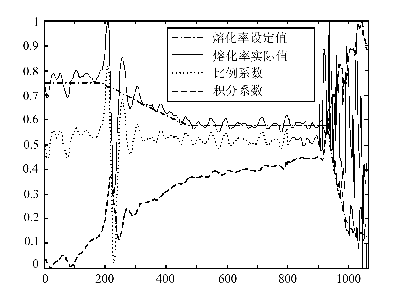
\includegraphics[width=6cm]{Image/01.eps}} 
	\vskip 1mm{\small
	图1\quad 熔化率与比例、积分系数之间的关
	\\
	Fig.\,1\quad Comparing melting rate with proportion and integral parameters of the Consarc controller }
	}
	}
\end{center}






\TeX 的参考文献的引用比较方便,比如我们想引用Knuth的The \TeX
book,可以输入``The \TeX book\verb|$^{[1]}$|''得到想要的效果``The
\TeX book$^{[1]}$''.再比如我们输入``\verb|多模态优化问题\,\!$^{[2]}$|''得到想要的效果``多模态优化问题\,\!$^{[2]}$''.

\subsection{作者简介注意事项}

文章末页需附作者中英文简介,简介不超过100字,包括作者姓名、职称、学习工作经历,以及研究方向.


作者照片请选用简单背景的证件照片,比例要求是$5:4$,大小做成3.0\,cm\,$\times$\,2.4\,cm.

在无照片情况下,采用biographynophoto环境来填写作者简历.
与正常情况的区别是,此时没有了照片文件这个参数.

\section{其他注意事项}

1) 因本刊文章为国内外公开发表,所有录用后稿件必须在本单位经保密审查.
修改加工后的定稿除根据录用通知要求发送一份至编辑部指定电子邮箱外,
另请一式两份,注明原稿件编号后附本单位同意公开发表的介绍信寄至编辑部.
如无特殊原因,录用通知发出半年后才收到的修改稿,本刊不再发表.

2)
请作者仔细地按照录用通知和该模版中的各项要求认真加工修改稿,若修改稿不符合要求,编辑部将退回作者重新修改直至合乎要求为止,
由此造成的稿件不能及时发表的责任由作者自负.
作者如无特殊声明,本刊默认第一作者为通信作者.
如果第一作者非文章通信作者或通信作者联系方式变动,
务请及时通知编辑部.


\end{multicols}%开始通栏显示
\vskip1mm
\hrule
\begin{equation}
T_{N-i}(m_{N-i})= \left[ \underbrace{O,\cdots,
O}_{Z_1^{N-i}(m_{N-i})} \underbrace{I \cdot h^{N-i}(n^{N-i}), I
\cdot h^{N-i}(n^{N-i}-1),\cdots, I \cdot
h^{N-i}(m^{N-i})}_{L^{(N-i)}},\underbrace{O,\cdots,
O}_{Z_2^{N-i}(m_{N-i})} \right]\tag{3}
\end{equation}
\begin{equation} \left[
  \begin{array}{c}
    \hat{{\pmb x}}(k+1) \\
    {\pmb e}(k+1)\\
  \end{array}
\right]=\left[
  \begin{array}{cc}
    A_0+B_0F+L_o(C(k)-C_0) & L_oC(k) \\
    (A(k)-A_0)+(B(k)-B_0)F-L_o(C(k)-C_0) & A(k)-L_oC(k) \\
  \end{array}
\right]\left[
  \begin{array}{c}
    \hat{{\pmb x}}(k) \\
    {\pmb e} (k)\\
  \end{array}
\right]\tag{4}
\end{equation}
\begin{multicols}{2}%开始双栏显示

\end{multicols}%开始通栏显示

\begin{center}
\vbox{\centering{\small 表1\quad 这是一个通栏的表格示例
\\
Table 1 \quad An exampletable in one column } \vskip2mm
\renewcommand{\baselinestretch}{1.2}
{\footnotesize\centerline{\tabcolsep=15pt\begin{tabular*}{\textwidth}{ccccc}
\toprule
对手 (OPP)                   & 比分 (CSU : OPP) & 团队决策所占比例 & 个体决策所占比例 & 团队决策与个体决策比值 \\
\hline
Cyberoos2001                &       3:0     &       71.5       &       28.5       &          2.51          \\
FCPortugal2001              &       1:0     &       68.4       &       31.6       &          2.16          \\
Gemini                      &      26:0     &       59.7       &       40.3       &          1.48          \\
Harmony                     &       3:0     &       69.9       &       30.1       &          2.32          \\
Lazarus                     &      11:0     &       57.3       &       42.7       &          1.34          \\
MRB                         &       2:0     &       63.2       &       32.8       &          1.93          \\
SBCe                        &       4:1     &       65.8       &       34.2       &          1.92          \\
UvA\_Trilearn\_2001         &       1:0     &       54.9       &       44.1       &          1.24          \\
UTUtd                       &      10:0     &       70.7       &       29.3       &          2.41          \\
WrightEagle2001             &       3:1     &       66.2       &       33.8       &          1.96          \\
Average                     &               &       64.8       &       35.2       &          1.84          \\
\bottomrule
\end{tabular*}}}}\end{center}

\begin{multicols}{2}%开始双栏显示
\begin{center}
{\centerline{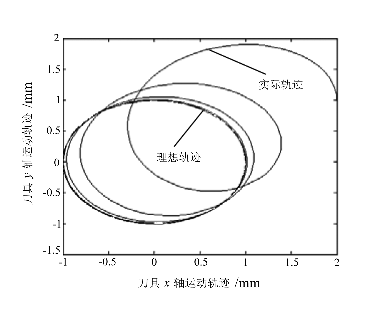
\includegraphics[width=6cm]{Image/02a.eps}}
{\footnotesize (a)控制参数1\\(a) Controller parameter 1}} \\
{\centerline{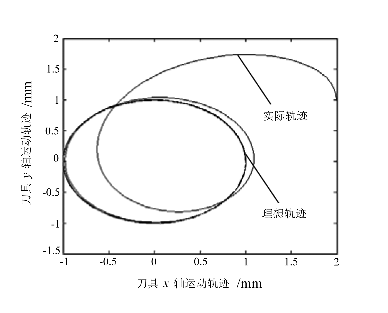
\includegraphics[width=6cm]{Image/02b.eps}} {\footnotesize
(b)控制参数2\\(b) Controller parameter 2}} \vskip1mm {\small
图2\quad 控制器参数对刀具运动轨迹的影响
\\Fig.\,2\quad The influences
of the controller parameters on the tracking errors}
\end{center}

3)
稿件经编辑加工和排版后,编辑部将把pdf校样通过E-mail发送给通信作者,请务必逐字逐句核对并在三天内返回校样.
除编辑和排版错误外请勿对校样内容作进一步的修改.
校样内容的修改将导致因需要请同行专家对稿件作进一步评议而延误文章发表,因此而导致的后果和发生的费用将由作者承担.

4) 在修改稿加工格式方面若有其他不明事宜,请来函来电垂询. 感谢合作!

\section{结论}

文章的结论请勿与摘要、前言等重复.

\section*{致谢}

文章作者可以在此处对支持和帮助其研究工作或本文写作的其他组织或人员表示感谢.
注意,支持此研究的基金项目请直接标注在首页页脚处,不用在此再次致谢.

\begin{thebibliography}{99}
\zihao{6} \addtolength{\itemsep}{0.2em} \urlstyle{rm}
\bibitem{1} Ran B, Boyce D E. {\sl Modeling Dynamic Transportation Network}.
Berlin: Springer-Verlag, 1996. 69$-$83

\bibitem{2} Payton D, Estkowski R, Howard M. Compound behaviors in pheromone robotics. {\sl Robotics and Autonomous Systems}, 2003, {\bf 44}(3): 229$-$240

\bibitem{3} Su Lian-Cheng, Zhu Feng. Design of a novel omnidirectional stereo vision system. {\sl  Acta Automatica Sinica}, 2006,{\bf 32}(1): 67$-$72\\ (苏连成, 朱枫. 一种新的全向立体视觉系统的设计. 自动化学报, 2006, {\bf 32}(1): 62$-$72)

\bibitem{4} Roychoudhury R, Bandyopadhyay S, Paul K. Adistributed mechanism for topology discovery in ad hoc wireless networks using mobile agents. In: Proceedings of IEEE First Annual Workshop on Mobile and Ad hoc Networking and Computing. NewYork, USA: IEEE, 2000. 145$-$146
 \bibitem{5} Hryniewicz O. An evaluation of the reliability of complex systems using shadowed sets and fuzzy lifetime data. {\sl International Journal of Automation and Computing}, to be published
 
 \bibitem{6} Zhang W. Reinforcement Learning for Job-Shop Scheduling [Ph.\,D.
dissertation], Peking University, 1996

\bibitem{7} The Math Works.Image Processing Toolbox for Use with Matlab: User$'$s Guide [Online], available: http://www.mathworks.com, November 3, 2006

\bibitem{8} Reily R C, Mack J L. The Self-organization of Spatially Invariant
Representations, Technical Report PDP.CNS.92.5, Department of
Psychology, Mellon University, USA, 1993

\bibitem{9} Wilkinson J P. Nonlinear Resonant Circuit, U.\,S. Patent 362412, July 1990

\bibitem{10} IEEE Criteria for Class IE Electric System, IEEE Standard 308, 1969

\bibitem{11} IEEE Criteria for Class IE Electric System, IEEE Standard 308, 1969
\bibitem{12} IEEE Criteria for Class IE Electric System, IEEE Standard 308, 1969
\end{thebibliography}

\begin{biography}[Image/ssl.eps]
\noindent{\hei
尚书林
}\quad
中国科学院自动化研究所博士研究生.
2002年获得北京师范大学信息学院电子系学士学位.
主要研究方向为图像与视频压缩技术.\\E-mail: aas\_editor@ia.ac.cn

\noindent({\bf
SHANG Shu-Lin
}\quad
Ph.\,D. candidate at the
Institute of Automation, Chinese Academy of Sciences. He received
his bachelor degree from Beijing Normal University in 2002. His research
interest covers image compression and video coding.)
\end{biography}

\begin{biography}[Image/nmzuo.eps]
\noindent{\hei
左年明
}\quad
中国科学院自动化研究所博士研究生.
2002年获得山东大学数学学院学士学位.
主要研究方向为医学图像处理, CT图像重建.\\E-mail: aas\_editor@ia.ac.cn

\noindent({\bf
ZUO Nian-Ming
}\quad
Ph.\,D. candidate at the
Institute of Automation, Chinese Academy of Sciences. He received
his bachelor degree from Shandong University in 2002. His research
interest covers medical CT image reconstruction and medical image
processing.)
\end{biography}

\begin{biographynophoto}
\noindent{\hei 陈培颖}\quad 《国际自动化与计算杂志》编辑部责任编辑.\\E-mail: peiying.chen@ia.ac.cn

\noindent({\bf CHEN Pei-Ying}\quad Managing editor at the Editorial Office of
{\sl International Journal of Automation and Computing}.)
\end{biographynophoto}

\begin{biographynophoto}
\noindent{\hei 欧\hskip2.5mm彦}\quad 《自动化学报(英文版)》编辑部责任编辑.\\E-mail: yan.ou@ia.ac.cn

\noindent({\bf OU Yan}\quad Managing editor at the Editorial Office of
{\sl IEEE/CAA Journal of Automatica Sinica (JAS)}.)
\end{biographynophoto}

\begin{biography}[Image/zz.eps]
\noindent{\hei
张\hskip2.5mm哲
}\quad
《国际自动化与计算杂志》与《自动化学报》编辑部技术编辑. 2006年获得北京工业大学电控学院自动化系学士学位.
本文通信作者.\\E-mail: zhe.zhang@ia.ac.cn

\noindent({\bf
ZHANG Zhe
}\quad
Copy-editor at the Editorial Office of
{\sl International Journal of Automation and Computing}, and {\sl
Acta Automatica Sinica}. He received his bachelor degree from Beijing
University of Technology in 2006. Corresponding author of this paper.)
\end{biography}
\end{multicols}
\end{document}
